\documentclass[xcolor=dvipsnames]{beamer}

\usepackage{graphicx}
\usepackage{listings}
\usepackage{comment}
\usepackage{float}

\usetheme{Frankfurt}
%\usecolortheme[named=OliveGreen]{structure}
%\usefonttheme{serif}
\setbeamertemplate{navigation symbols}{}
\setbeamertemplate{frametitle}[default][center]

\begin{document}
\title{A Bidirected String Graph Model of Genome Assembly}
\author{Eric Biggers}
\institute{Macalester College}
\date{December 5, 2012}
%\titlegraphic{\includegraphics[scale=0.3]{pineapple.jpg}}

\frame{\titlepage}

\begin{frame}{Genomes}
	\begin{itemize}
		\item A genome (for our purposes) is a long string of A's, C's, G's, and T's
		\item Dual-stranded
		\begin{itemize}
			\item A pairs with T and C pairs with G
			\item The two strands run in opposite directions
		\end{itemize}
	\end{itemize}
	\begin{center}
	{\tt $\leftarrow$ GTTGCTATAAATACGGGTCATGGTATTTTAGTACCG $\leftarrow$ \\}
	{\tt $\rightarrow$ CAACGATATTTATGCCCAGTACCATAAAATCATGGC $\rightarrow$}
	\end{center}
	\begin{itemize}
		\item Each letter in the genome is also known as a {\bf base pair}
		(abbreviation: bp)
	\end{itemize}
	\begin{table}[H]
		\caption{Genome sizes of selected organisms}
		\begin{tabular}{|c|c|c|}
			\hline
			E. coli (a common bacterium) &  ~4,600,000 bp \\
			\hline
			Ananas comosus (pineapple) &	~500,000,000 bp \\
			\hline
			Homo sapiens (human)       &  ~3,000,000,000 bp \\
			\hline
		\end{tabular}
	\end{table}
\end{frame}

\begin{frame}{Genome Sequencing}
	\begin{itemize}
		\item How can we deteremine the precise sequence (in terms of A's, T's,
		C's, and G's) of an organism's genome?

		\item Currently available sequencing technologies can only sequence
		fragments a few dozen to a few thousand bp long

		\item Genome assembly:
			\begin{itemize}
				\item Lab work
				\begin{enumerate}[1.]
						\item Obtain a DNA sample
						\item Break DNA into much smaller fragments
						\item Sequence the fragments using available technology
				\end{enumerate}
				\item Computational Work
				\begin{enumerate}[4.]
					\item Given the sequenced fragments, reconstruct the original genome.
				\end{enumerate}
			\end{itemize}
	\end{itemize}
\end{frame}

\begin{frame}{Reads}
	\begin{itemize}
		\item A {\bf read} is a short sequence of the letters A, C, T, G that
		represents some DNA that was sequenced by the sequencing machine.
		\item A read may come from any location on the genome, from either
		strand.
		\item Reads from opposite strands go in opposite directions.
			\begin{itemize}
				\item As a result, a sequence and its {\bf reverse-complement}
				(the corresponding sequence on the other strand, going
				backwards) are usually considered equivalent.
			\end{itemize}
	\end{itemize}
\end{frame}


\begin{frame}{Genome assemblers}
	\begin{itemize}
		\item An {\bf assembler} is a program or algorithm that can put together the
		``puzzle'' to reconstruct the original genome.
		\item  Input: a set of reads (lengths: ~35 to 5000bp each).
		\item  Output: one strand of the reconstructed genome (if possible)--- but
		in general, an exact answer may be impossible, so the output must be a set
		of substrings of the original genome that are as long as possible. (lengths:
		~10,000 to 10,000,000bp each).
	\end{itemize}
\end{frame}

\begin{frame}{Genome assembly vs Shortest Common Supersequence}
	Genome assembly is superficially similar to the shortest common superstring
	(SCS) problem, which is to find the shortest string that contains all strings
	from a given set.
	\begin{center}
	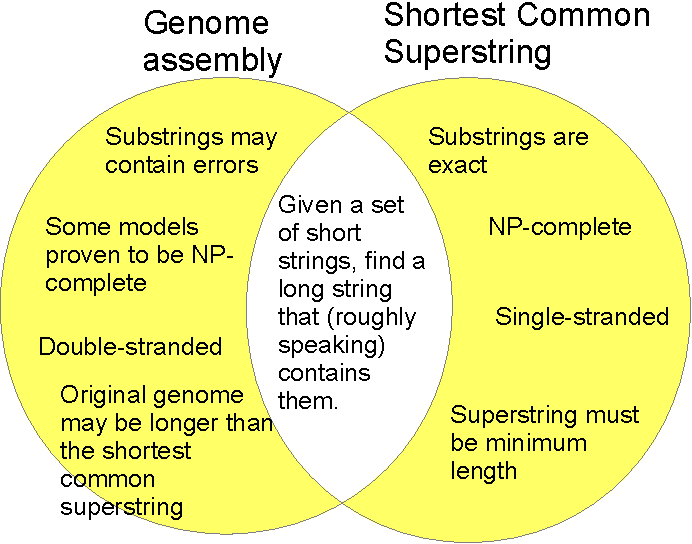
\includegraphics[scale=0.6]{venn-crop.pdf}
	\end{center}
\end{frame}

\begin{frame}{Ideas for genome assembly algorithms}

	\begin{itemize}
		\item Use the reads to build a graph that models the assembly problem.
		\item Find paths through the graph to reconstruct the original sequence.
	\end{itemize}
\end{frame}


\begin{frame}{Overlaps between reads}

	\begin{itemize}
	\item Two reads that overlap are likely to come from adjacent positions on the genome.
	\end{itemize}

	{\tt Read 1: \ \ \ \ \ \ \ \ \ $\rightarrow$ ATATAT\textcolor{red}{GCTGGTTACTT} $\rightarrow$ } \\
	{\tt Read 2: \ \ \ \ \ \ \ \ \ \ \ \ \ \ \ 
		$\rightarrow$ \textcolor{red}{GCTGGTTACTT}TGATAGATA $\rightarrow$ } \\
	{\tt Possible genome: $\rightarrow$ ATATATGCTGGTTACTTTGATAGATA $\rightarrow$}

	\begin{itemize}
	\item Overlapped reads may be from different strands.  Note the different
	directions of the two reads here.  The overlapped regions of the two reads
	are {\bf reverse-complement} from each other.
	\end{itemize}

	{\tt Read 1: \ \ \ \ \ \ \ \ \ 
			$\rightarrow$ ATATAT\textcolor{red}{GCTGGTTACTT} $\rightarrow$ } \\
	{\tt Read 2: \ \ \ \ \ \ \ \ \ \ \ \ \ \ \ 
			$\leftarrow$ \textcolor{red}{CGACCAATGAA}ACTATCTAT $\leftarrow$ } \\
	{\tt Possible genome: $\rightarrow$ ATATATGCTGGTTACTTTGATAGATA $\rightarrow$}
\end{frame}


\begin{frame}{Computing overlaps}
	\begin{itemize}
		\item Compute all pairwise overlaps of some minimum length $\ell$ among the
		reads.
		\item Naive algorithm compares every read with every other read ($N$
		reads: $N^2$ time)
		\item A faster algorithm indexes the reads by short subsequences, then only
		compares reads that share a subsequence ("seed-and-extend").
		\item Overlaps may be exact, or they may allow for differences up to a
		certain threshold.
		\item Implementation: {\tt compute-overlaps}
			\begin{itemize}
				\item Input:  A set of reads and the minimum overlap length
				\item Output:  All exact pairwise overlaps between reads,
				including reverse-complement overlaps
				\item Algorithm:  Seed-and-extend
			\end{itemize}
	\end{itemize}
\end{frame}

\begin{frame}{Build the fragment string assembly graph}
	\begin{itemize}
		
		\item Use the overlaps as evidence to construct a graph modeling the assembly.
		\item Each vertex represents a read.
		\item Each edge represents an overlap.
		\item Two reads are connected with an edge iff they share an overlap.
		\item A {\it string graph} is a graph where the edges are labeled with
		strings.
		\item In this case, each edge is labeled with DNA sequence of the {\em
		non-overlapped region} (this will be explained later)
		\item Should the edges be directed or undirected?
	\end{itemize}
\end{frame}


10. Bidirected graphs

- At this stage, we don't actually know which strands the reads are from!

------------>            or             <------------
     <-------------             -------------->

- We must allow the edges to be traversed in either the forward or
  reverse-complement direction... but each read MUST be used in a consistent way
  in the reconstruction.

- A _bidirected graph_ is a graph where a directed head is attached to both
  edges.

- There are 3 (or 4, ignoring symmetry) types of bidirected edges.  They follow
  directly from the different types of overlaps.

     ------->   ------>      ------>     <------
  <-------         <-------     ------>     <------

      |               |           |          |
      V               V           V          V  

  <--------->   >---------<  >-------->  <--------<

- In this example, two vertices (reads) may have multiple _bidirected edges_
  between them if they overlap in different ways, but there can be at most one
  _bidirected edge of the same type_ between two vertices if we always prefer
  the best overlap of a given type.

\begin{comment}

11. Walking through the bidirected string graph

- A _walk on a bidirected graph_ is a continuous sequence of edges such that
  if we enter a vertex v through a head inwards, we leave it on a head outwords,
  and vice versa.

- A bidirected edge may be traversed in opposite directions.

- The reverse of a walk in a directed graph is also a bidirected walk.

    - Interpretation: one direction of the walk spells out the _forward_
      sequence.  The other direction spells out the _reverse complement_
      sequence.

12. Transitive reduction

- Very commonly, given three adjacent reads f, g, and h, f will overlap h as
  well as g.  This is redundant information because we can equivalently walk f
  ?-? g ?-? h, but the walks visiting more vertices are preferred because they are
  supported by more reads.

------------->
     -------------->
         --------------->

- Transitive reduction finds edges f ?-? h, described above, and removes them.
- Algorithm:  Go through each vertex and examine neighbors up to 2 steps away to
  identify all transitive edges leaving this vertex.  (Some optimizations are
  possible.)

13. Collapsing unbranched paths

Find unbranched paths and collapse them.

f >-> g >-> h >-> i >-> j >-> k

f >-< g <-> h >-< i <-< j <-> k

Ideally, most the genome will be unbranched sequence.  These sequences will be
assembled after this step of the algorithm.

But, real genomes contain repeats, and they will create branches in the graph.

14. Traversal count calculation

Estimate the traversal count of each edge.

Ideally, every edge will be traversed exactly one time.
- But, real genomes always contain repetitive sequence, and these regions may
appear multiple times in the final assembly.
- It is also possible for there to be erroneous parts of the graph that should
  not be included in the final assembly at all.

A-statistic formula

15. Minimum cost network flow

We need to determine how many times edge must be traversed.

Remember, some edges may be repeated sequence, and they therefore may appear
multiple times in the original genome.

Given the bidirected string graph with each edge labeled as OPTIONAL, EXACTLY
ONCE, or AT LEAST ONCE, compute a minimum-cost network flow that makes the graph
Eulerian.

16. Compute an Eulerian tour of the graph to produce a reconstruction of the
original genome.

A generalized Eulerian tour through the bidirected graph will produce a possible
reconstruction of the original genome.

- General case:  The original genome cannot be reconstructed in one piece, so
  the final reconstruction must take the form of the smallest set of paths that
  traverse all the edges the required number of times.

17. Implementation:

- A set of C++ programs that iteratively transform the data into the final
  assembly.
- Different sets of stages of the algorithm may be run in order to reach the
  final assembly.

Each node is a binary program.

The arrows indicate the output from one program being used in other program.


            convert-reads

                |
                V
                ...

Reads are input in textual form, e.g. the FASTA format:

>read_1
ATATTATATAT
>read_2
GCGCGTGTGTA

Genome is output in textual form.

A _contig_

>contig_1
TTTATAGTAGTAGTTGATTAGTATAGTGATGATAGTAGTA...

- Many things still would need to be improved to make this competitive with
  other assemblers.

18. References

- The Fragment String Assembly Graph (2005) by Eugene W. Myers
    * Main algorithm I have described.

- Maximum Likelihood Genome Assembly (2009) by Paul Medvedev and Michael Brudno
    * Explanation of bidirected graphs and bidirected graph algorithms applied
    * to DNA sequences.
\end{comment}

\end{document}
